%%%%%%%%%%%%%%%%%%%%%%%%%%%%%%%%%%%%%%%%%
% a0poster Portrait Poster for LiRI/UZH
% LaTeX Template
% Version 1.0 (22/06/13)
% Version 2.0 (08/04/22)
%
% The a0poster class was created by:
% Gerlinde Kettl and Matthias Weiser (tex@kettl.de)
% adapted by Danny McDonald for LiRI/UZH (mcddjx@gmail.com)
%
% License:
% CC BY-NC-SA 3.0 (http://creativecommons.org/licenses/by-nc-sa/3.0/)
%
%%%%%%%%%%%%%%%%%%%%%%%%%%%%%%%%%%%%%%%%%

\documentclass[a0,portrait]{a0poster}

% control margins here
\usepackage{geometry}
 \geometry{
 a0paper,
 left=5cm,
 top=4.5cm,
 right=5cm,
 bottom=1cm
 }
\addtolength{\textwidth}{4.5cm} % width of text can be adjusted if margins above are adjusted

\usepackage{multicol} % This is so we can have multiple columns of text side-by-side
\columnsep=3em % This is the amount of white space between the columns in the poster
\columnseprule=0pt % This is the thickness of the black line between the columns in the poster

% UZH colours
\usepackage[svgnames]{xcolor}
\definecolor{red100}{RGB}{204, 3, 1}
\definecolor{uzhblau80}{RGB}{51,83,183}
\definecolor{uzhockerrot100}{RGB}{220, 96, 39}
\definecolor{uzhockerrot80}{RGB}{227, 128, 82}
\definecolor{uzhflaschengruen100}{RGB}{42, 127, 98}
\definecolor{uzhflaschengruen80}{RGB}{86, 157, 133}
\definecolor{about}{RGB}{237,204,212} % 
\definecolor{conclusion}{RGB}{204,212,237} % the conclusion box colour
\usepackage{multirow}

\usepackage{ifthen} % needed to stop horizontal line above 'Conclusions' section
\usepackage{graphicx} % Required for including images
\graphicspath{{figures/}} % Location of the graphics files
\usepackage{mwe,tikz}\usepackage[percent]{overpic} % overlay your photo over the background
\usepackage{booktabs} % Top and bottom rules for table
\usepackage[font=small,labelfont=bf]{caption} % Required for specifying captions to tables and figures
\usepackage{amsfonts, amsmath, amsthm, amssymb} % For math fonts, symbols and environments
\usepackage{wrapfig} % Allows wrapping text around tables and figures
\usepackage{tgheros}
\renewcommand{\sfdefault}{qhv}
\renewcommand{\familydefault}{\sfdefault}

\usepackage[onehalfspacing]{setspace} % remove for single spacing
\usepackage{tcolorbox} % for the conclusions box
\usepackage{blindtext} % you can remove this once you add your content
\usepackage[export]{adjustbox} % allow floating a graphic right
\usepackage{titlesec} % customising section titles
\usepackage{needspace} % prevent break between line and section title
\usepackage{nameref} % package and command to get the name of the current section (for ifthen)
\usepackage[version=4]{mhchem}
\usepackage{tabularx}
\usepackage{booktabs}
\usepackage[official]{eurosym}
\newcolumntype{R}[1]{>{\raggedleft\arraybackslash}p{#1}}

\begin{document}

% define how our section titles will look (with ruled line)
\titleformat{\section}
  {\needspace{1\baselineskip}\sectionrule\huge\bfseries}
  {\color{red100}\thesection.}
  {1em}
  {\color{red100}}

% draw horizontal line before section unless it is conclusions (if you change name of Conclusions, you should
% also change it here too so it is recognised and the line suppressed
\makeatletter
\newcommand{\sectionrule}{%
 \ifthenelse{\equal{\@currentlabelname}{Conclusions}}
 % use the below line instead of the above if conclusions is a section*
 % \ifthenelse{\equal{\@currentlabelname}{}}
  {}
  {\vspace*{-\baselineskip}
  %  \vrule height 1pt depth 1pt width \linewidth\vskip0.4pt
   \bigskip}%
}
\makeatother


%----------------------------------------------------------------------------------------
%	POSTER HEADER 
%----------------------------------------------------------------------------------------
%\title{Creating a \LaTeX{} poster template matching UZH specifications for LiRI presentations}
\title{The Role of PCI-PMI Infrastructure in Reaching Europe's Energy Policy Targets}

% the top logo (in english!) and unit title
% \noindent

\noindent
\begin{minipage}[b][2cm][t]{0.753\linewidth} 
  % First Row
  \vspace{1em}
  \begin{minipage}{0.15\textwidth}
    
\includegraphics[height=3.5cm]{tub-logo.pdf}
  \end{minipage}
  \begin{minipage}{0.2\textwidth}
    
\includegraphics[height=4.5cm]{ensys-logo-en.pdf}
  \end{minipage}
  \vspace{2.3em}

  % Second Row
  \begin{minipage}{0.9\textwidth}
    \makeatletter
    \raggedright{\fontsize{75pt}{65pt}\selectfont\color{red100}\textbf{{\@title}}\par}
    \makeatother
    \color{Black}
    \vspace{0.3cm}
    \hspace{0.005em}
    resilient-project.github.io $\cdot$ pypsa.org $\cdot$ github.com/PyPSA/pypsa-eur $\cdot$ github.com/bobbyxng
  \end{minipage}
\end{minipage}%
%
\begin{minipage}[b][2cm][t]{0.3\linewidth} % Second minipage
    \begin{minipage}[t]{0.3\linewidth}
        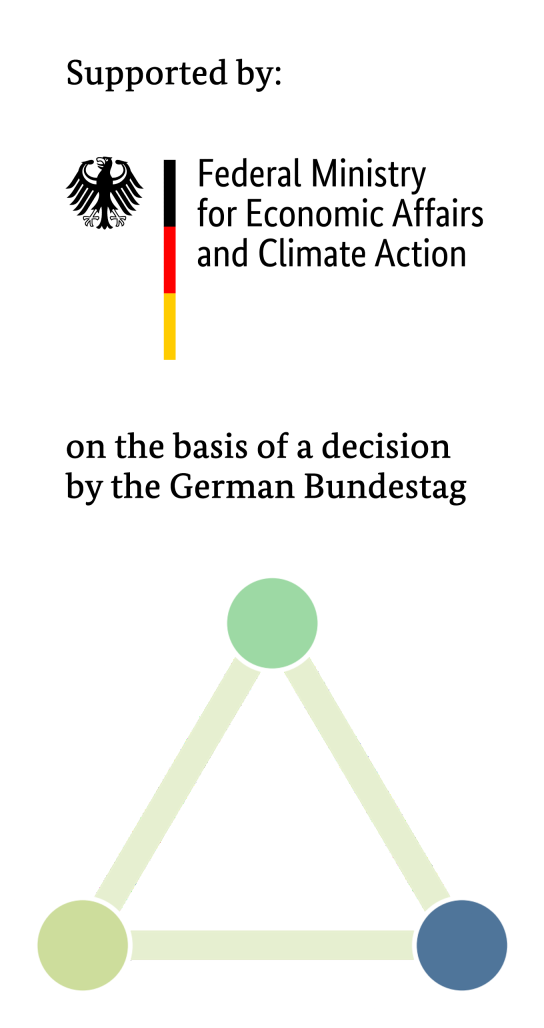
\includegraphics[height=13cm]{resilient_bmwk_logo.png}
    \end{minipage}
    \hfill
    \begin{minipage}[t]{0.7\linewidth}
        
\includegraphics[height=13cm]{qr.pdf}
    \end{minipage}%     
\end{minipage}

\vspace{14em}



%----------------------------------------------------------------------------------------
%	POSTER BODY
%----------------------------------------------------------------------------------------

\begin{multicols}{3}
\raggedcolumns

%----------------------------------------------------------------------------------------
%	PYPSA
%----------------------------------------------------------------------------------------

\noindent \textcolor{red100}{\huge \textbf{Motivation}}
\\
\textit{EU targets and PCI-PMI projects}
\\
\noindent
The European Union (EU) aims to achieve climate-neutrality by 2050, with ambitious domestic \ce{H2} production and \ce{CO2} sequestration targets next to a net-zero transition. The European Commission selects so-called Projects of Common Interest (PCI) and Projects of Mutual Interest (PMI) (Figure \ref{fig:regional_scope_map}) --- large infrastructure projects for electricity, hydrogen and \ce{CO2} transport, and storage --- that are of transnational importance as they link the energy systems of European countries.

\noindent
\begin{center}
    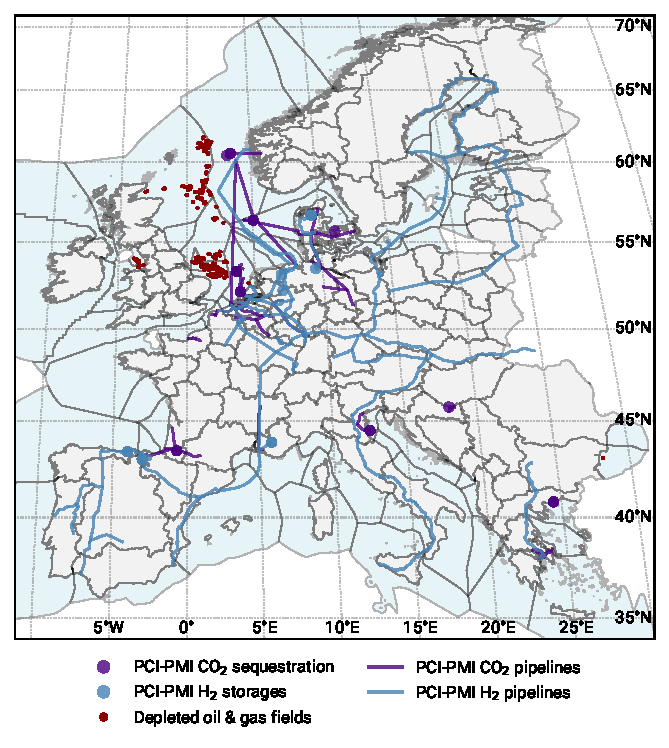
\includegraphics[width=0.90\linewidth]{map_adm_pcipmi.pdf}
    \captionof{figure}{Map of the regional scope including clustered onshore (grey) and offshore regions (blue), as well as PCI-PMI \ce{CO2} and \ce{H2} pipelines, storage and sequestration sites. Depleted offshore oil and gas fields (red) provide additional \ce{CO2} sequestration potential \cite{hofmannH2CO2Network2025}.}
    \label{fig:regional_scope_map}
\end{center}

\noindent In this work, we evaluate the impact of PCI-PMI projects for the European energy system and EU energy policies using a \textbf{regret-analysis} approach (Table \ref{tab:regret_matrix_setup}) using the open-source sector-coupled energy system model PyPSA-Eur \cite{hofmannH2CO2Network2025,horschPyPSAEurOpenOptimisation2018,neumannPotentialRoleHydrogen2023}. More specifically, we run five long-term scenarios varying in the degree of \ce{CO2} and \ce{H2} infrastructure deployment, including the on-time commissioning of PCI-PMI projects. In a second step, we evaluate the performance of these long-term scenarios in a short-term scenario (potential realisation), i.e. (i) reduced policy targets, (ii) delay of PCI-PMI, or (iii) no pipelines at all. In total, 60 optimisations are run at 2190 snapshots (on avg. 4h resolution) for 99 NUTS regions.

\vspace{2em}

\begin{center}
    \captionof{table}{Regret matrix setup: Long-term and short-term scenarios.}
    \label{tab:regret_matrix_setup}
    \scriptsize
    \begin{tabularx}{\linewidth}{R{7.5cm}>{\centering\arraybackslash}X>{\centering\arraybackslash}X>{\centering\arraybackslash}X}
        \toprule
        \textbf{Short-term} & \textbf{Reduced targets} & \textbf{Delayed pipelines} & \textbf{No pipelines} \\
        \midrule
        \textbf{Long-term scenarios} & & & \\
        Decentral Islands (\textbf{DI}) & $\blacksquare$ & -- & -- \\
        PCI-PMI (\textbf{PCI}) & $\blacksquare$ & $\blacksquare$ & $\blacksquare$ \\
        PCI-PMI nat. (\textbf{PCI-n}) & $\blacksquare$ & $\blacksquare$ & $\blacksquare$\\
        PCI-PMI internat. (\textbf{PCI-in}) & $\blacksquare$ & $\blacksquare$ & $\blacksquare$ \\
        Central Planning (\textbf{CP}) & $\blacksquare$ & $\blacksquare$ & $\blacksquare$ \\
        \midrule
        \textbf{Targets} & & & \\
        GHG emission reduction &  $\blacksquare$ &  $\blacksquare$ &  $\blacksquare$ \\
        \ce{CO2} sequestration &  -- &  $\blacksquare$ &  $\blacksquare$ \\
        Electrolytic \ce{H2} production &  -- &  $\blacksquare$ &  $\blacksquare$ \\
        \ce{H2} electrolysers &  -- &  $\blacksquare$ &  $\blacksquare$ \\
        \midrule
        \textbf{\ce{CO2} + \ce{H2} infrastructure} & & & \\
        \ce{CO2} sequestration sites & $\blacksquare$ &  $\blacksquare$ &  $\blacksquare$ \\
        \ce{CO2} pipelines to seq. site & $\blacksquare$ &  $\blacksquare$ &  $\blacksquare$ \\
        \ce{CO2} pipelines & $\blacksquare$ &  $\square$ &  -- \\
        \ce{H2} pipelines & $\blacksquare$ &  $\square$ &  -- \\
        \bottomrule
    \end{tabularx}
    $\blacksquare$ enabled \quad $\square$ delayed by one period \quad -- disabled
\end{center}
\vspace{2em}

\noindent
\begin{center}
  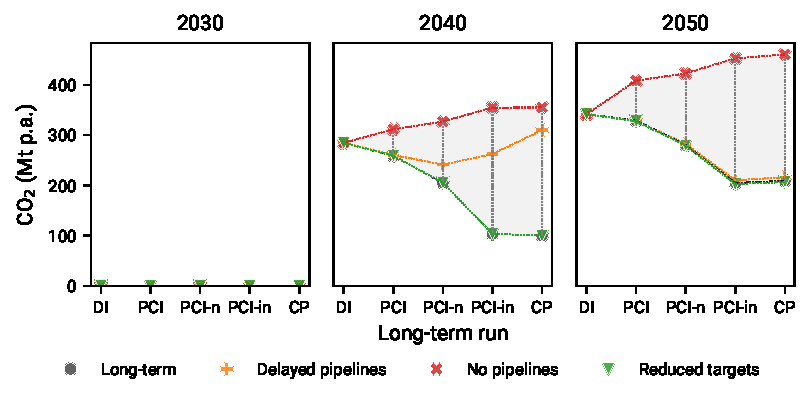
\includegraphics[width=\linewidth]{delta_balances_DAC.pdf}
  \captionof{figure}{DAC utilisation}
  \label{fig:dac_balance}
\end{center}
\vspace{2em}

\columnbreak

\noindent \textcolor{red100}{\huge \textbf{Key results}}
\\
\textit{Pipelines vs. DAC}

\noindent In the \textit{PCI} scenario, \textbf{\ce{CO2} pipelines} transport \ce{CO2} from biomass-based industry process and point sources equipped with carbon capture in north-western Europe to sequestration sites in the North Sea (Figure \ref{fig:PCI-in_lt_2050_co2}). These include PCI-PMI projects (around 114 Mt p.a.) and up to 286 Mt p.a. of additional potential from depleted oil and gas fields.

\begin{center}
    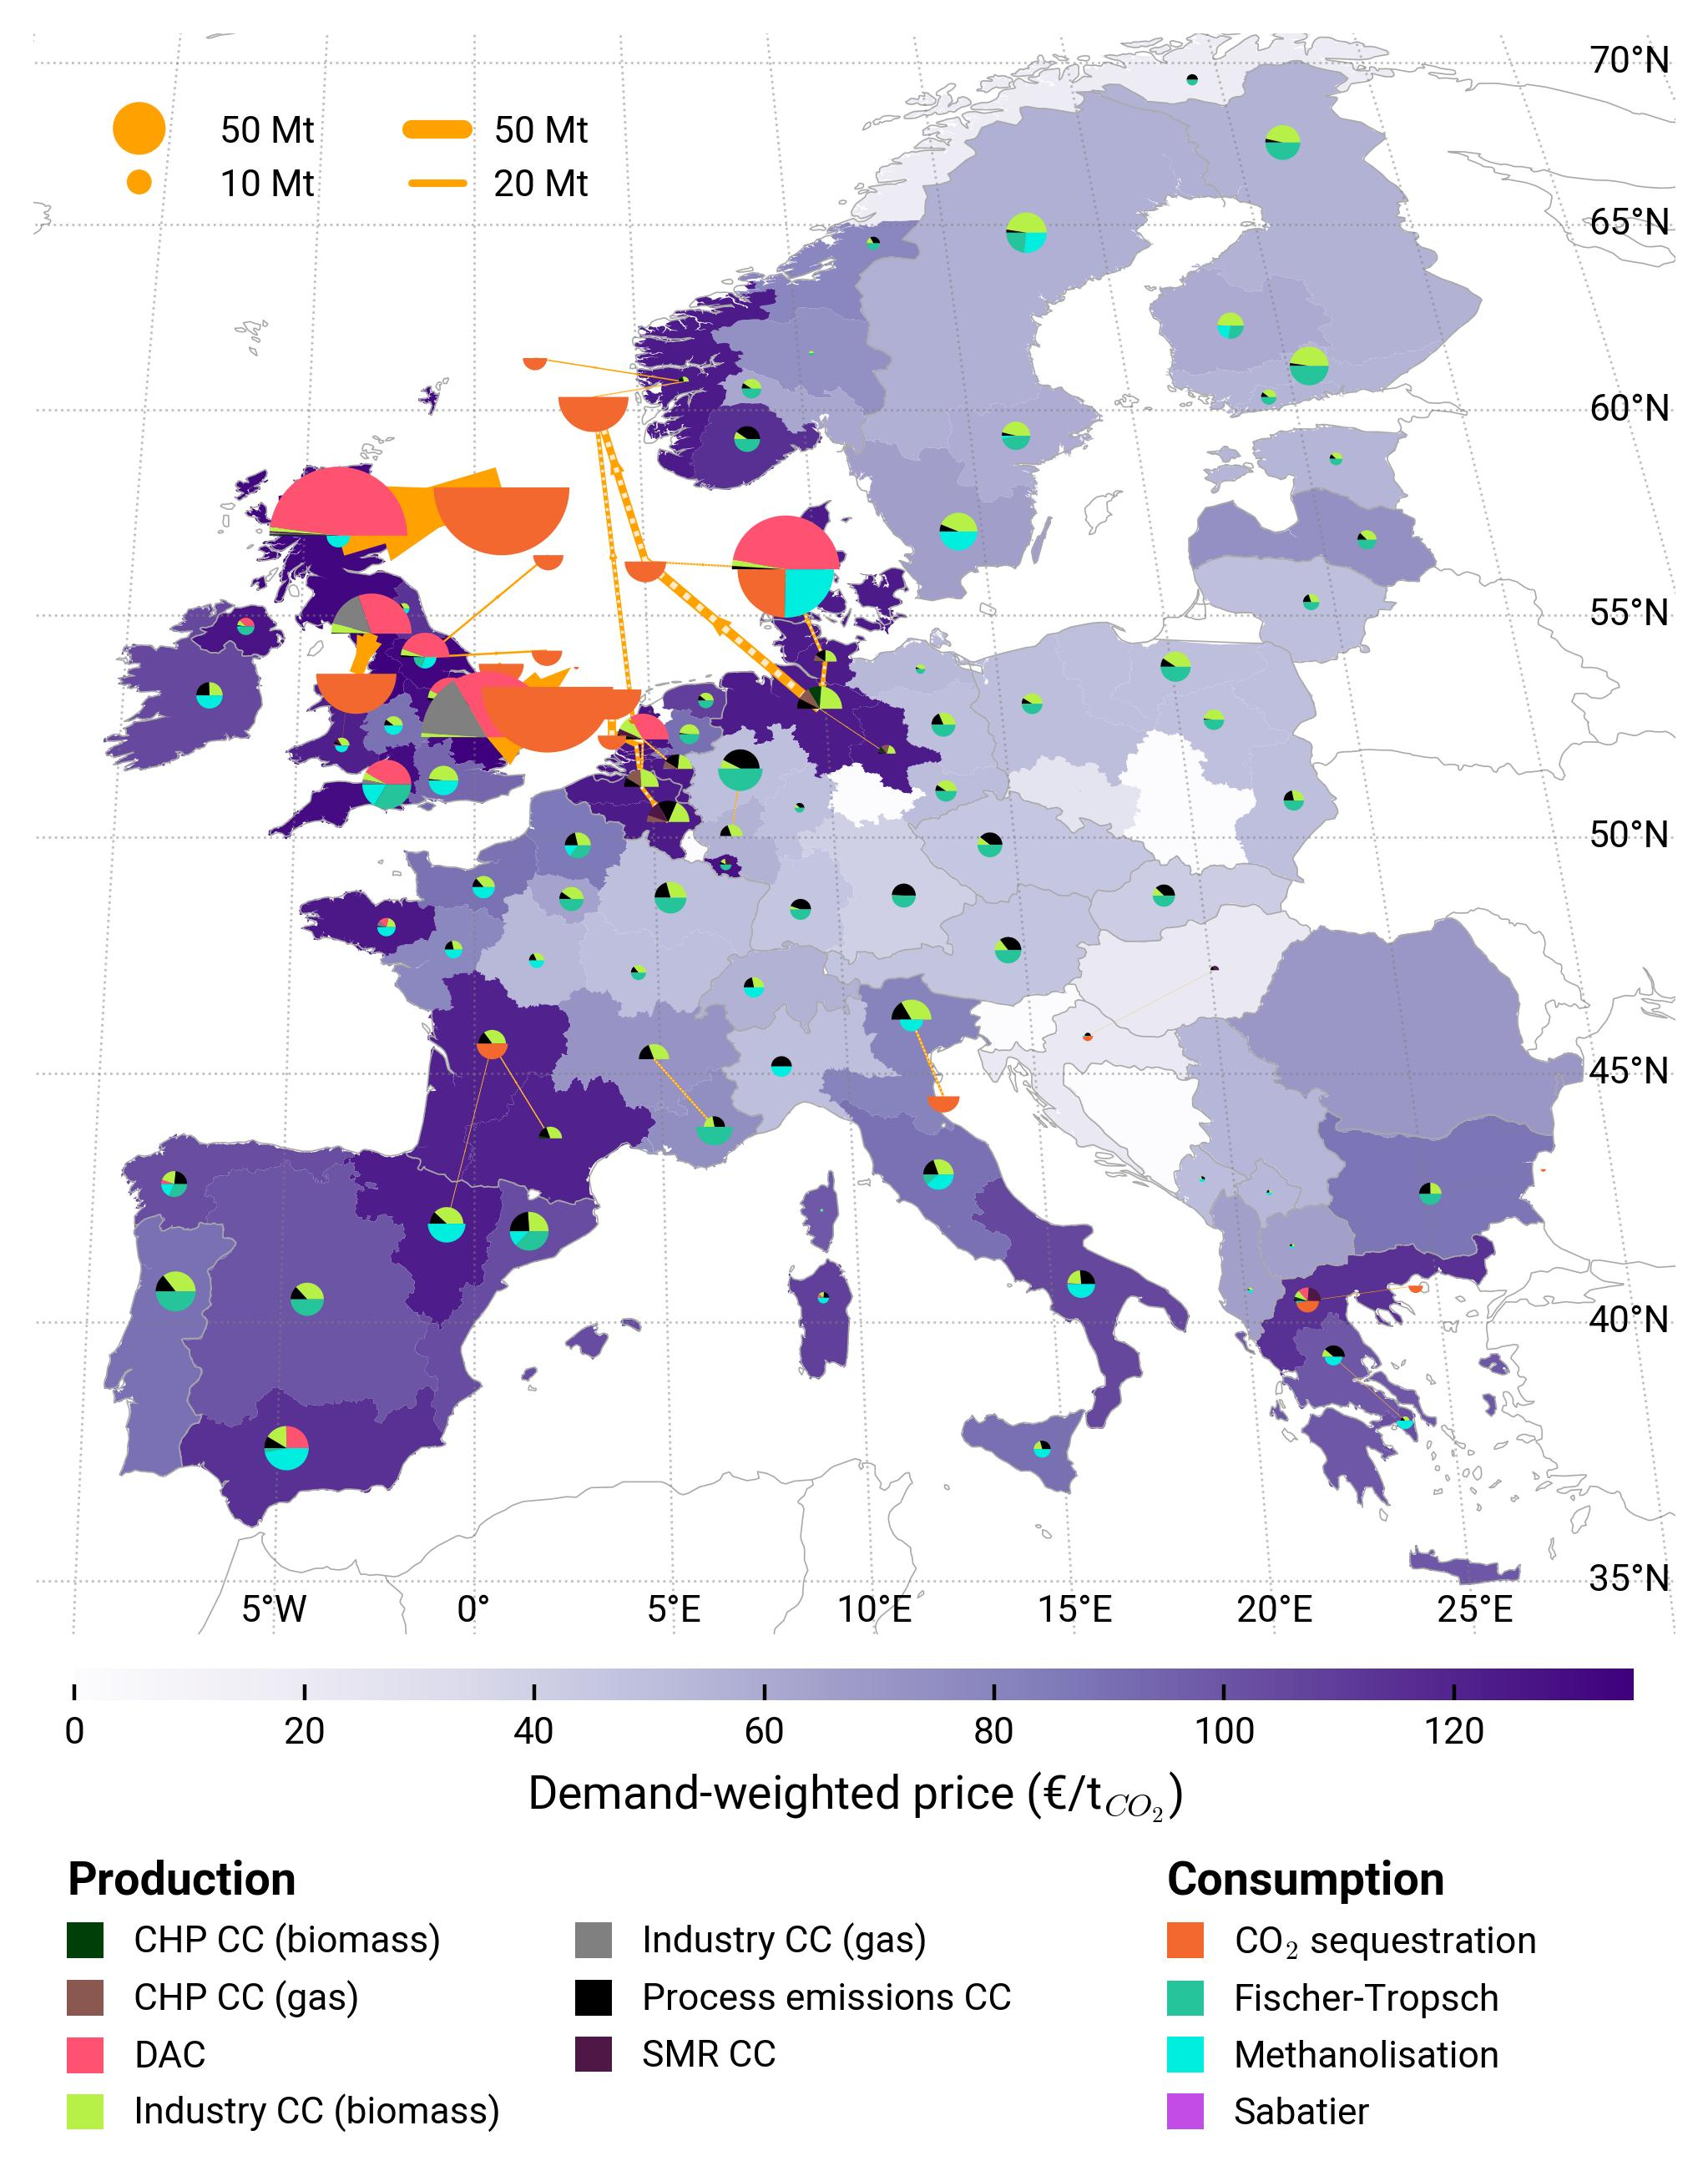
\includegraphics[width=\linewidth]{base_s_adm___2050-balance_map_co2_stored.jpg}
    \captionof{figure}{\textit{PCI} long-term scenario (2050) --- \ce{CO2} balances and distribution}
    \label{fig:PCI-in_lt_2050_co2}
\end{center}
\vspace{2em}
\noindent Results show that a build-out of \ce{CO2} pipelines \textbf{reduces the reliance on expensive DAC technology} (Figure \ref{fig:dac_balance}). Seeing a delay in the commissioning of pipeline projects leads to a significant increase in the use of DAC, most visible in the year 2040. In the most extreme case, DAC utilisation in pipeline scenarios by up to 300 Mt p.a. if the pipelines are not built at all, and the system has to react on short notice through additional investments or higher utilisation of existing assets.

\noindent \textbf{\ce{H2} pipelines} connect production sites at locations with high renewable energy potential to demand sites, e.g. for methanol and Fischer-Trosch synthesis or direct use in the industry (Figure \ref{fig:PCI-in_lt_2050_h2}).

\begin{center}
    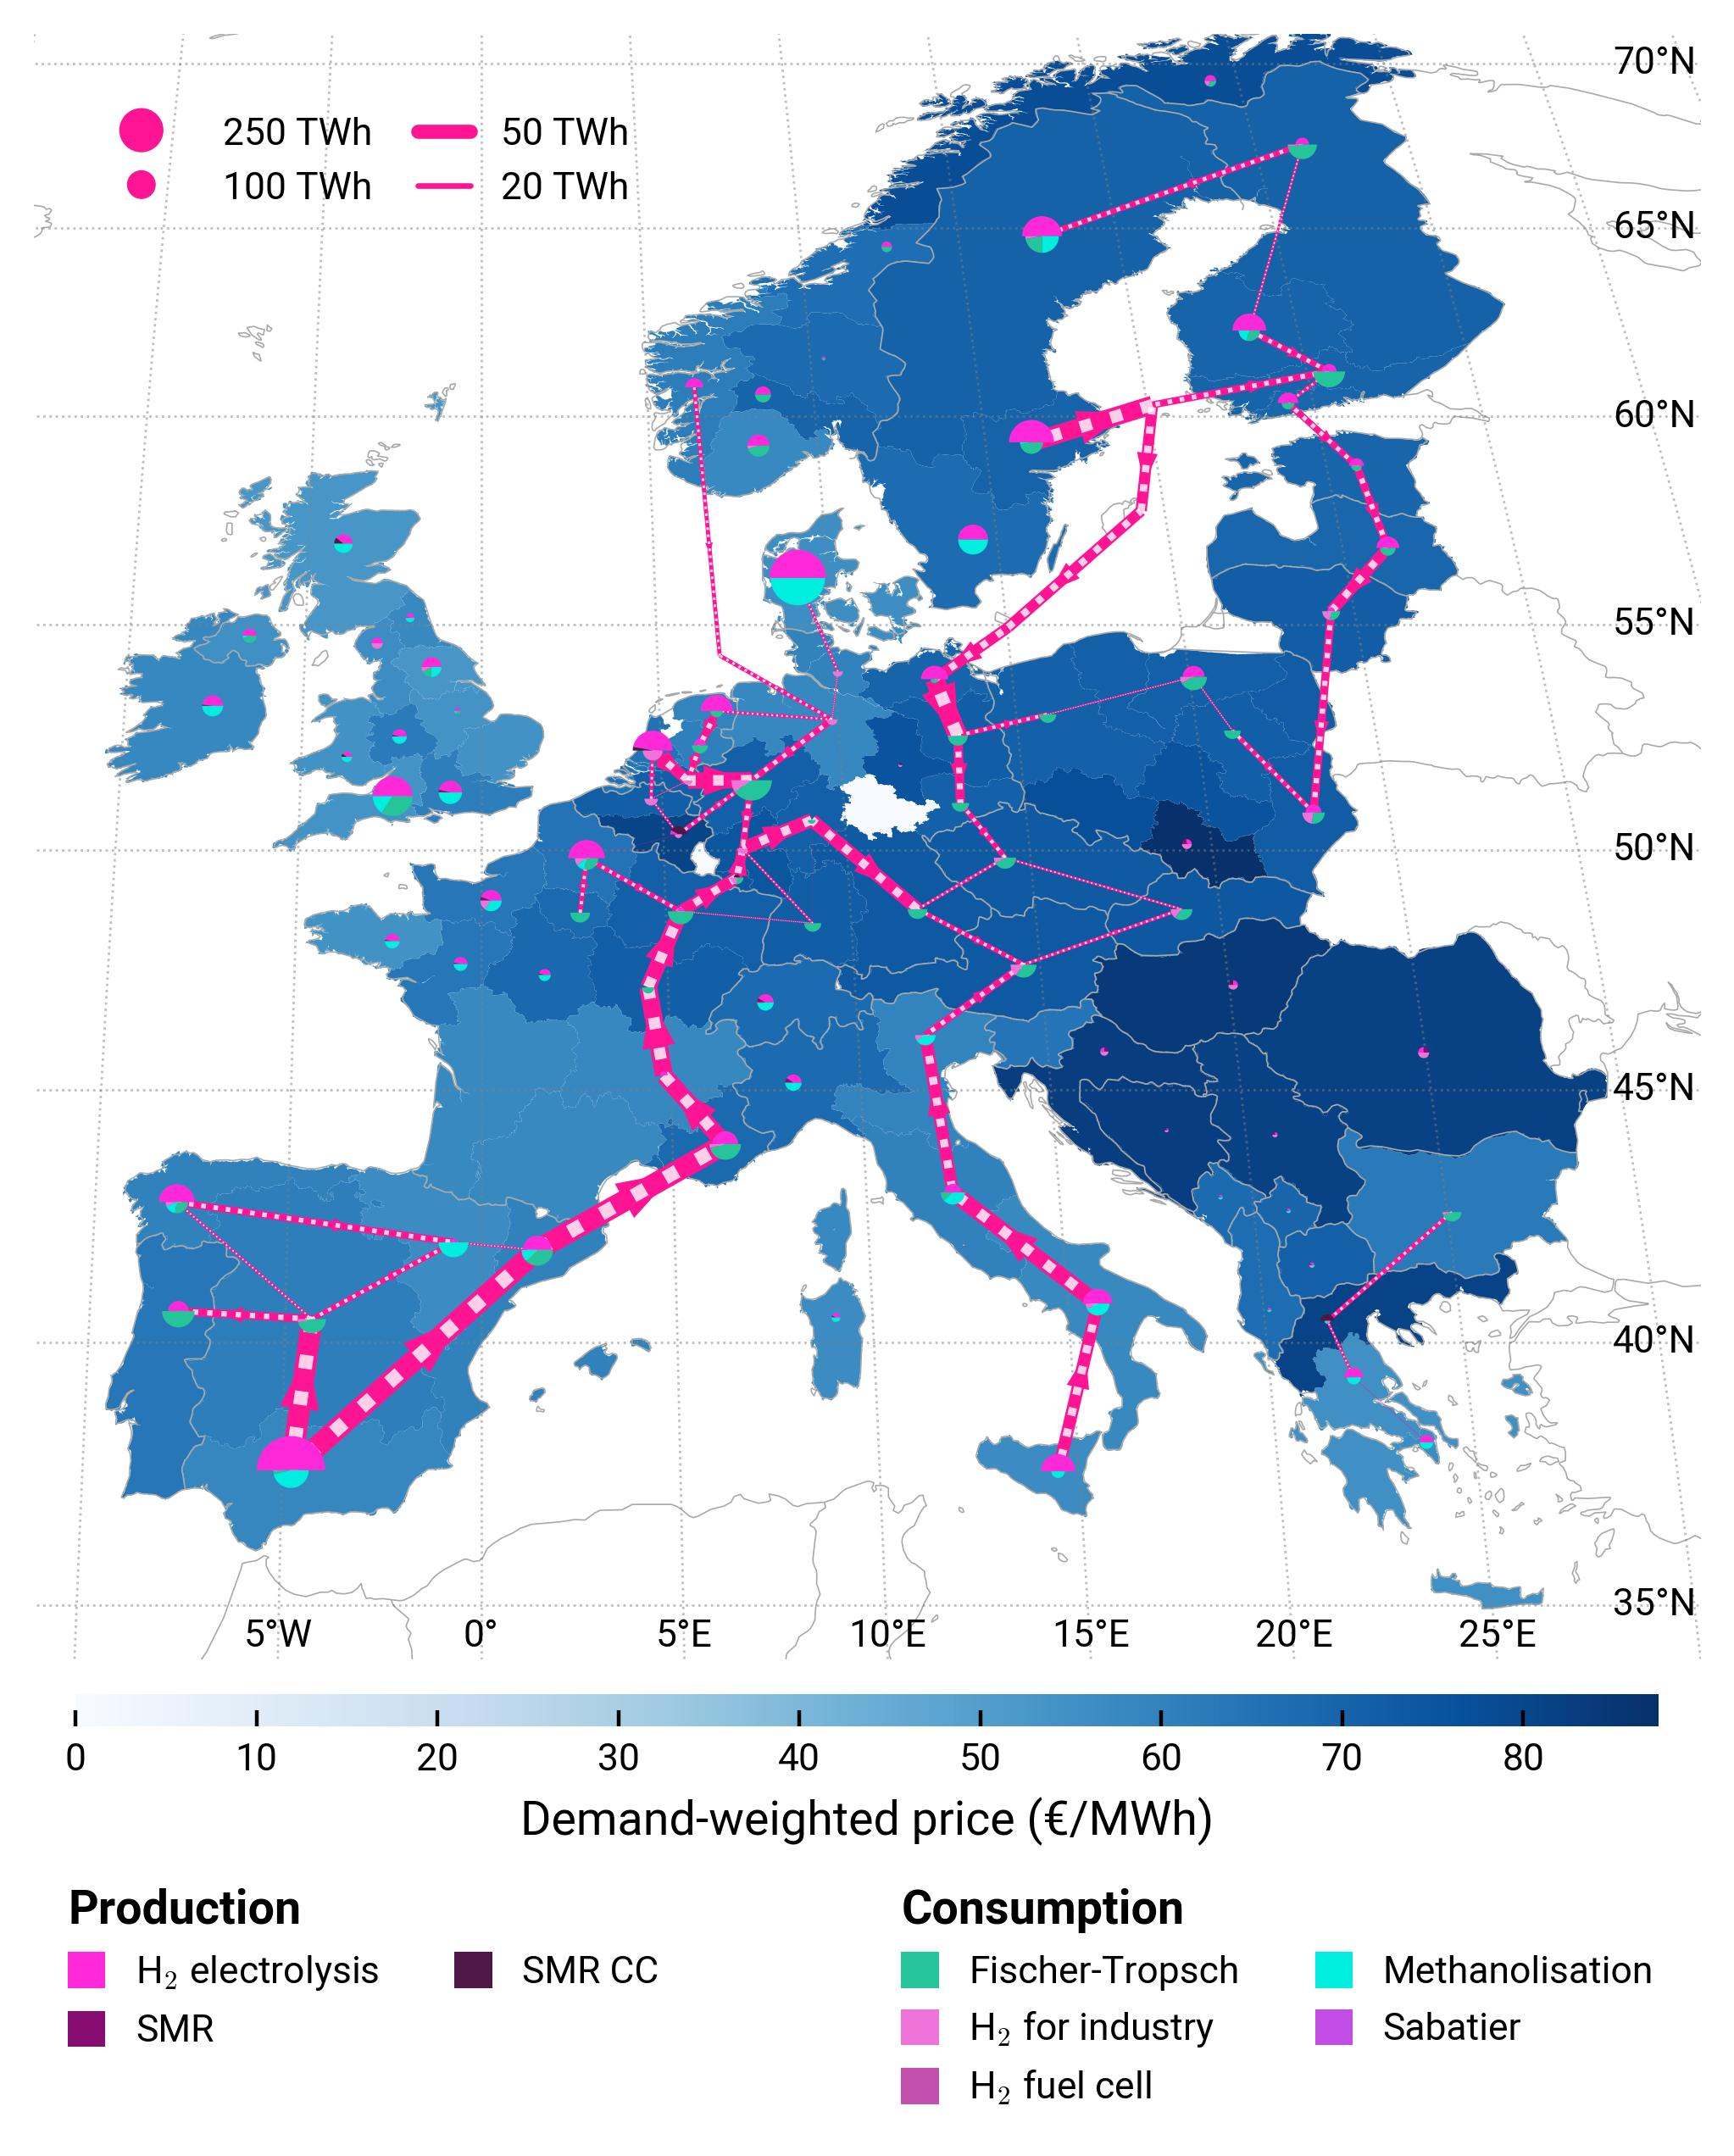
\includegraphics[width=\linewidth]{base_s_adm___2050-balance_map_H2.jpg}
    \captionof{figure}{\textit{PCI} long-term scenario (2050) --- \ce{H2} balances and distribution}
    \label{fig:PCI-in_lt_2050_h2}
\end{center}




% \noindent \textcolor{red100}{\huge \textbf{PyPSA}}
% \\
% \textit{Python for Power System Analysis}
% \\

% \noindent
% PyPSA is an open-source toolbox for \textbf{simulating and optimising modern power and energy 
% systems} that include features such as conventional generators with unit commitment, 
% variable wind and solar generation, storage units, coupling to other energy sectors, 
% and mixed alternating and direct current networks. \\

% \noindent \textcolor{black}{\large \textbf{Functionality}}

% \noindent PyPSA can calculate:

% \begin{itemize}
%     \item static power flow (using both the full non-linear network equations and the linearised network equations)
%     \item linear optimal power flow (least-cost optimisation of power plant and storage dispatch within network constraints, using the linear network equations, over several snapshots)
%     \item security-constrained linear optimal power flow
%     \item total electricity/energy system least-cost investment optimisation
% \end{itemize}

\columnbreak
%----------------------------------------------------------------------------------------
%	SECTIONS
%----------------------------------------------------------------------------------------
\noindent \textcolor{red100}{\huge \textbf{Take-aways}}
\\
\textit{Preliminary}
\begin{itemize}
  \item PCI-PMI \ce{CO2} and \ce{H2} pipelines support reaching the European policy targets at lower costs, especially over the total lifetime of the assets (Figure \ref{fig:system_costs}).
  \item More pipeline investments unlock even higher system cost savings of additional 7-16 bn. \euro{} p.a. in 2050 by reducing the reliance on expensive DAC technology.
  \item Delays of projects in 2030 barely affect total system costs. However, delays of PCI projects in combination with endogenous pipeline investments can increase system costs by up to 35.2 bn \euro{} p.a. (Figure \ref{fig:regret_matrix}).
\end{itemize}

\vspace{0.5em}
\begin{center}
    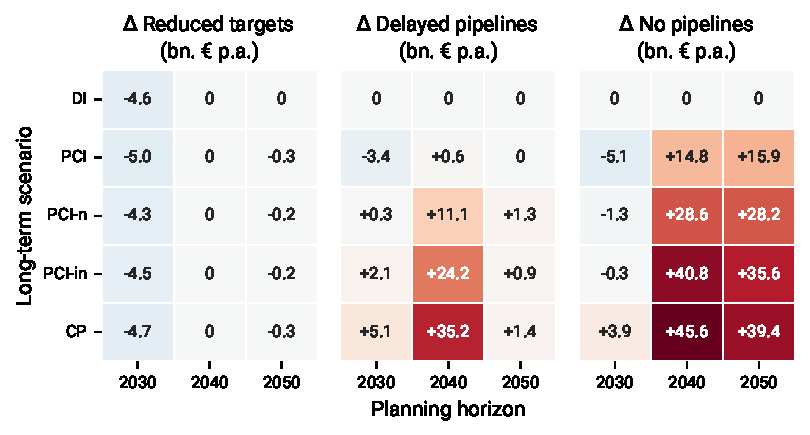
\includegraphics[width=\linewidth]{regret_matrix.pdf}
    \captionof{figure}{Regret matrix. Calculating regret terms by subtracting system costs of long-term scenarios (columns) from short-term scenarios (rows). Positive values reflect higher costs in the short-term scenarios compared to the long-term ones.}
    \label{fig:regret_matrix}
\end{center}
\vspace{0.5em}

\begin{center}
  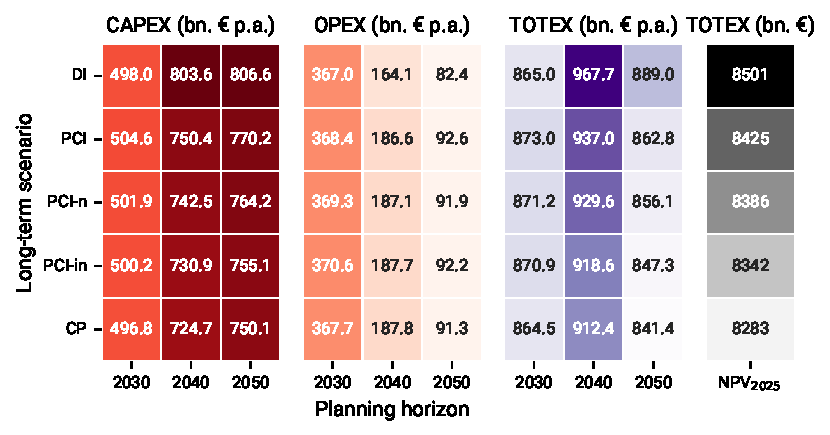
\includegraphics[width=\linewidth]{totex_heatmap.pdf}
  \captionof{figure}{Total system costs}
  \label{fig:system_costs}
\end{center}
\vspace{2em}

\noindent \textcolor{red100}{\huge \textbf{RESILIENT project}}
\\

\noindent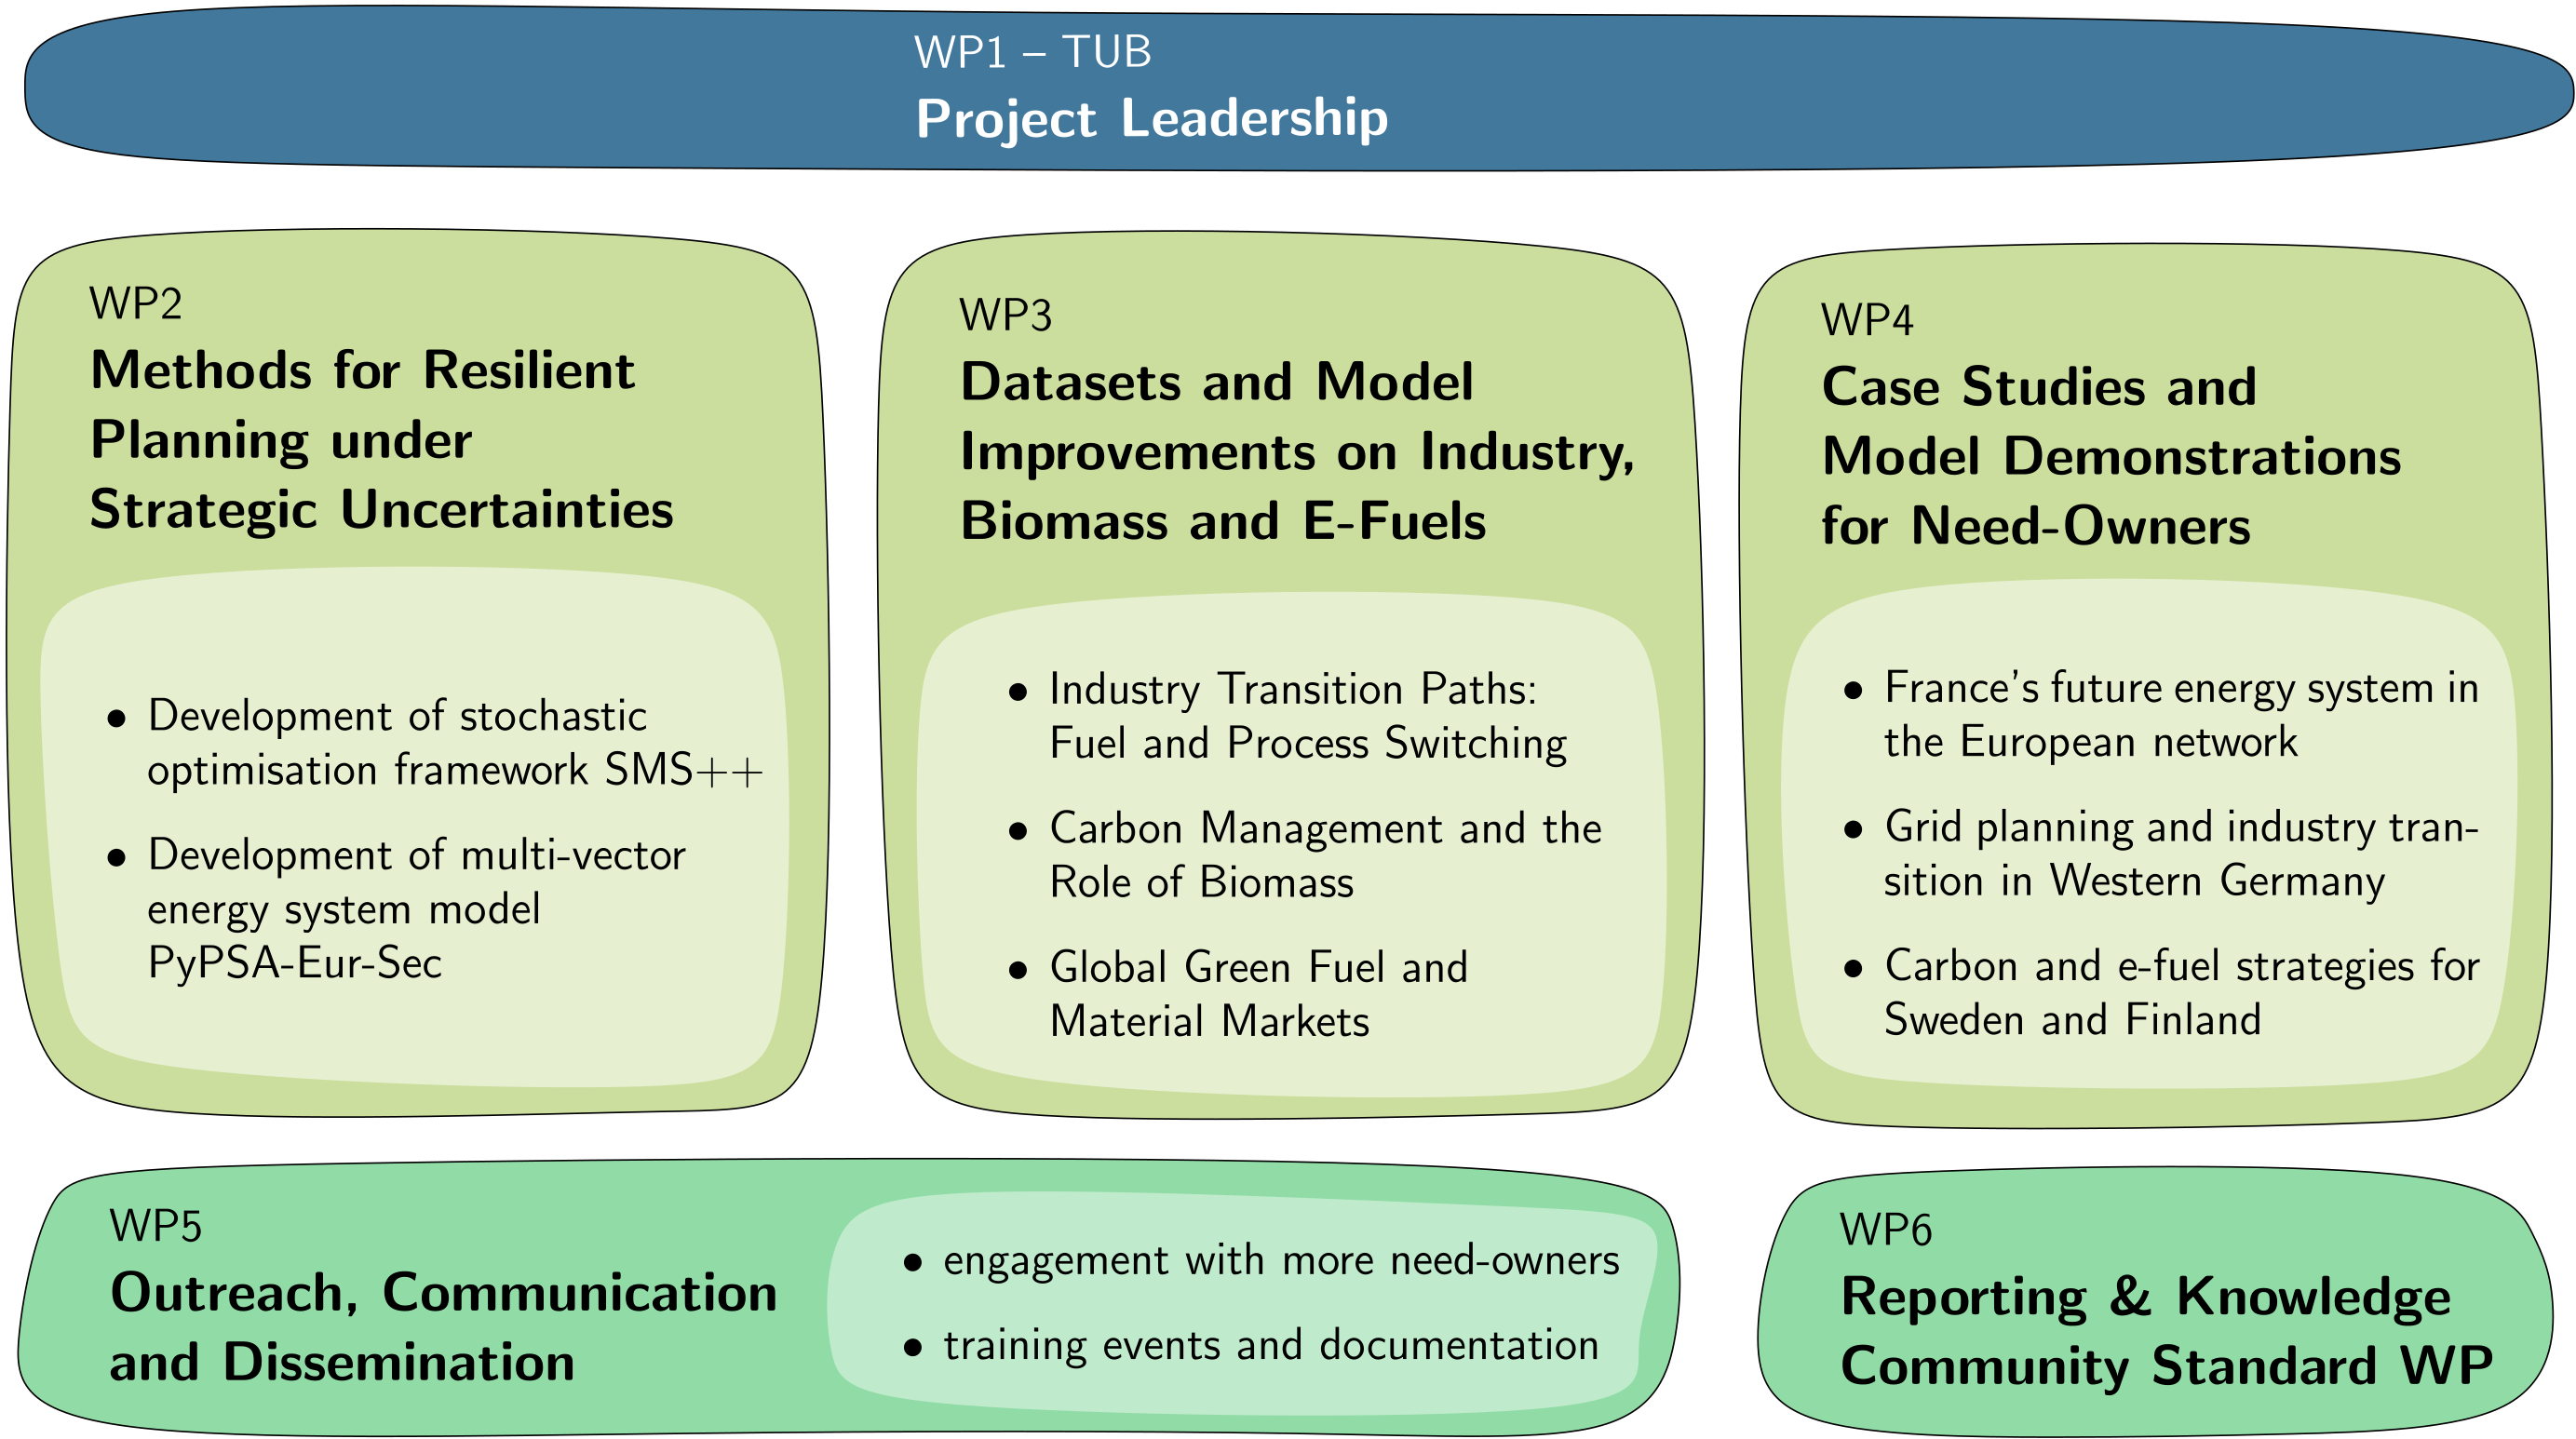
\includegraphics[width=\linewidth]{resilient_project_structure.png}

\noindent This work was supported by the German Federal Ministry for Economic Affairs and Climate Action (BMWK) under Grant No. 03EI4083A (RESILIENT). This project has been funded by partners of the CETPartnership (https://cetpartnership.eu) through the Joint Call 2022. As such, this project has received funding from the European Union's Horizon Europe research and innovation programme under grant agreement no. 101069750.

%---------------------------------------------------------------------------------------
%	REFERENCES
%---------------------------------------------------------------------------------------

\singlespacing
\small
% \nocite{*} % Print all references regardless of whether they were cited in the poster or not
\bibliographystyle{plain} % Plain referencing style
\bibliography{references}



%---------------------------------------------------------------------------------------
\end{multicols}

% Add keywords and author in footer minipage
\vfill % pushes footer to bottom if space allows

\begin{center}
  \colorbox{red100}{\parbox{1\linewidth}{
    \centering
    \color{white}
    \textbf{Contact:} Bobby Xiong (xiong@tu-berlin.de) \quad
    \textbf{Keywords:} open-source $\cdot$ energy system modelling $\cdot$ policy targets $\cdot$ infrastructure $\cdot$ resilience $\cdot$ hydrogen $\cdot$ carbon $\cdot$ Europe 
  }}
\end{center}

\end{document}